% id: 0335
% book: RPM 미적분Ⅱ · 03 지수함수와 로그함수의 미분
% section: 유형 UP 14 지수함수·로그함수의 극한의 도형에의 활용
% figure: crop:fig-0335.png
% answer: ④
% answer_source: 답지(쪽 렌더)
% variant_level: 0 (원본 전사)
% 이 파일은 build.mjs 가 items.json 에서 만든다. 고칠 때는 items.json 을 고친다.
\smash{\raisebox{4.5mm}{\dmkichul{RPM 미적분Ⅱ 0335번 · 51쪽}}}
\noindent\begin{minipage}[t]{0.58\linewidth}\vspace{0pt}\raggedright 오른쪽 그림과 같이 직선 $x=t\ (t>0)$가 곡선 $y=2e^{2x}-2$와 만나는 점을~$\pt{P}$, $x$축과 만나는 점을~$\pt{Q}$라 할 때, $\displaystyle\lim_{t\to 0+}\dfrac{\seg{PQ}}{\seg{OQ}}$의 값은? \cond{$\pt{O}$는 원점이다.}\end{minipage}\hfill\begin{minipage}[t]{0.4\linewidth}\vspace{0pt}\centering \setlength{\dmfigw}{82.2pt}\ifdim\dmfigw>\linewidth\setlength{\dmfigw}{\linewidth}\fi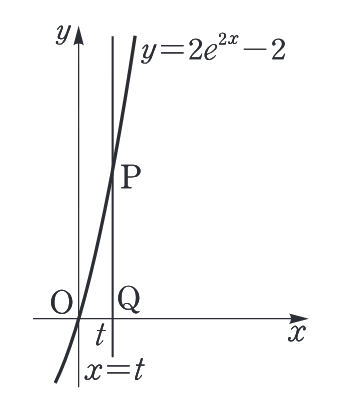
\includegraphics[width=\dmfigw]{figures/fig-0335.png}\end{minipage}\par
\begin{choicesii}{$1$}{$2$}{$3$}{$4$}{$5$}\end{choicesii}
